\documentclass[tikz,border=5pt]{standalone}
\usepackage{amssymb,amsmath}
\begin{document}
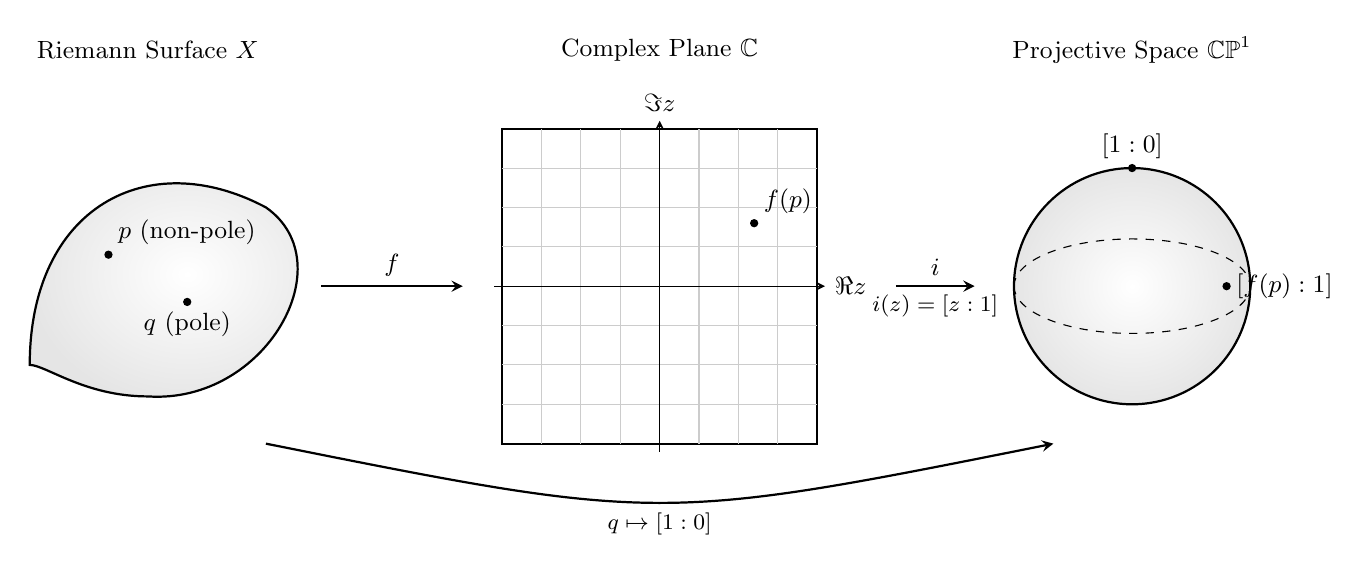
\begin{tikzpicture}[font=\small,>=stealth]
%----------------------------
% Left: Riemann surface X (smooth patch)
%----------------------------
\begin{scope}[shift={(-6,0)}]
	% Surface patch for X
	\shade[inner color=white, outer color=gray!20, draw=black, thick]
	(-2,-1) .. controls (-2,1) and (-0.5,1.8) ..
	(1,1)   .. controls (2,0.3) and (1,-1.5) ..
	(-0.5,-1.4) .. controls (-1.3,-1.4) and (-1.8,-1) ..
	cycle;
	\node at (-0.5,3) {Riemann Surface $X$};
	
	% non-pole p
	\fill (-1,0.4) circle (1.5pt)
	node[above right] {$p$ (non-pole)};
	
	% pole q
	\fill (0,-0.2) circle (1.5pt)
	node[below] {$q$ (pole)};
\end{scope}
	
%----------------------------
% Middle: Complex plane C (with grid)
%----------------------------
\begin{scope}
	% Draw a square region for C
	\draw[thick] (-2,-2) rectangle (2,2);
	\node at (0,3) {Complex Plane $\mathbb{C}$};
	
	% Light grid inside
	\foreach \x in {-1.5,-1,...,1.5}
	\draw[gray!40] (\x,-2) -- (\x,2);
	\foreach \y in {-1.5,-1,...,1.5}
	\draw[gray!40] (-2,\y) -- (2,\y);
	
	% Axes
	\draw[->] (-2.1,0) -- (2.1,0) node[right] {\(\Re z\)};
	\draw[->] (0,-2.1) -- (0,2.1) node[above] {\(\Im z\)};
	
	% image of p under f
	\fill (1.2,0.8) circle (1.5pt) node[above right] {\(f(p)\)};
	
%	% suggest f(q) "goes to infinity"
%	\draw[->,densely dashed] (0.7,-0.7) -- (1.7,-1.7);
%	\node at (1.9,-1.9) {\footnotesize ``$\infty$''};
\end{scope}

%----------------------------
% Right: CP^1 as a sphere
%----------------------------
\begin{scope}[shift={(6,0)}]
	% Sphere for CP^1
	\shade[inner color=white, outer color=gray!20, draw=black, thick]
	(0,0) circle (1.5);
	\node at (0,3) {Projective Space $\mathbb{CP}^1$};
	% Equator (to suggest the affine chart)
	\draw[dashed] (-1.5,0) arc (180:360:1.5 and 0.6);
	\draw[dashed] (-1.5,0) arc (180:0:1.5 and 0.6);
	
	% north pole = [1:0]
	\fill (0,1.5) circle (1.5pt);
	\node[above] at (0,1.5) {$[1:0]$};
	
	% equator point = [f(p):1]
	\fill (1.2,0) circle (1.5pt);
	\node[right] at (1.2,0) {$[f(p):1]$};
	
	% note affine chart below
%	\node at (0,-2.0) {\footnotesize affine chart \(\{[z_0:z_1]\mid z_1\neq 0\}\)};
\end{scope}

%----------------------------
% Arrows: f, F, inclusion i
%----------------------------
% arrow f: X -> C (from p)
\draw[->,thick]
(-4.3,0) -- (-2.5,0)
node[midway, above] {$f$};

%%% arrow F: X -> CP^1 (from p)
%\draw[->,thick]
%(-4.3,-2) .. controls (0,-5) .. (3.8,-2)
%node[midway,above] {$F$};

% image of pole q under F: q -> [1:0]
\draw[->,thick]
(-5,-2) .. controls (0,-3) .. (5,-2)
node[midway, below] {\footnotesize \(q\mapsto [1:0]\)};

% inclusion i: C -> CP^1, z |-> [z:1]
\draw[->,thick]
(3,0) -- (4,0)
node[midway,above] {$i$};
\node at (3.5,-.25) {\footnotesize \(i(z)=[z:1]\)};
	
\end{tikzpicture}
\end{document}
